158. \begin{figure}[ht!]
\center{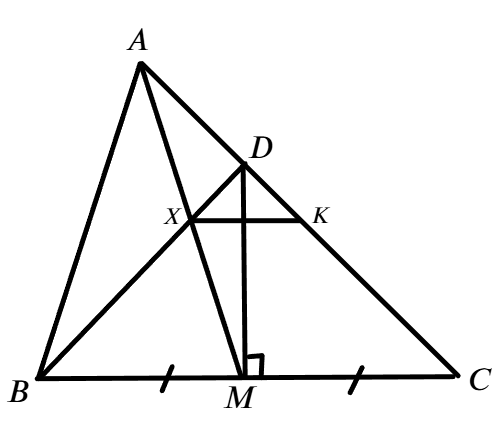
\includegraphics[scale=0.35]{g7-155.png}}
\end{figure}\\
В треугольнике $BDC$ высота $DM$ совпадает с медианой, значит он равнобедренный и $BD=DC.$ Пусть $K$ --- середина стороны $AC,$ тогда $KC=\cfrac{1}{2} AC=BX,$ откуда имеем равенство $DX=BD-BX=DC-KC=DK.$ Значит, треугольник $DXK$ также является равнобедренным. Заметим, что $\angle DKX=\cfrac{180^\circ-\angle DXN}{2}=\angle DCB,$ поэтому прямые $XK$ и $BC$ параллельны, так как равны соответственные углы при секущей $XK.$ В треугольнике $MAC$ отрезок $XK$ параллелен основанию $BC$ и проходит через середину стороны $AC,$ а значит является его средней линией и $X$ является серединой стороны $AM,$ ч.т.д.\\
